\documentclass[12pt]{support/thcolognethesis} 

\usepackage{amssymb}

\title{Optimierung von Augmented Reality Anwendungen durch die Berücksichtigung von Tiefeninformationen mit Googles Project Tango}

\degree{Masterthesis}

\author{Steffen Tröster}

\college{
	Technischen Hochschule Köln\\
    Ingenieurwissenschaftliches Zentrum\\
    Fakultät für Informations-,\\
    Medien- und Elektrotechnik}

\course{Technische Informatik (Master)}

\company{inovex GmbH}  

\firstExaminer{Prof. Dr. Martin Eisemann}
\firstExaminerLocation{Technische Hochschule Köln}
\secondExaminer{Christian Meder}
\secondExaminerLocation{inovex GmbH}

\degreedate{Köln, im \monthyeardate\today}
	
\begin{document}

\baselineskip=18pt plus1pt

\setcounter{secnumdepth}{3}
\setcounter{tocdepth}{2}

\maketitle                 

\begin{abstract}
\setlength{\parskip}{1em}

Project Tango ist eine neue mobile Plattform des Google Advanced Technology and Project (ATAP) Teams, die in der Lage ist, Bewegungsverfolgung, Tiefenwahrnehmung und Umgebungswiedererkennung auf Smartphones und Tablets anbieten zu können. Durch die kontinuierliche Bestimmung der relativen Geräteposition eignet sich die Plattform besonders für dreidimensionale Augmented Reality (AR) Anwendungen. Die Illusion dieser AR Anwendungen wird besonders dann gestört, wenn sich reale Objekte in einer Szene räumlich vor virtuellen Objekten befindet und diese virtuellen Objekte nicht entsprechend ausgespart werden. 

Diese Arbeit stellt daher drei Überdeckungsverfahren vor, mit denen diese Überlagerung der virtuellen Objekte mit Hilfe der Tiefenwahrnehmung von Project Tango und des Z-Buffer Algorithmus realisiert werden kann. Die Tiefeninformationen für den Z-Buffer werden hierfür zum einen direkt aus den Sensordaten und alternativ mit einer TSDF Rekonstruktion und einer selbst zusammengestellten Ebenen Rekonstruktion bestimmt. Außerdem wird auf einen zusätzlichen Ansatz eingegangen, der zur Verbesserung dieser Tiefeninformationen die Bildinformationen der Farbkamera durch den Guided Filter berücksichtigt. Diese Mechanismen werden im Laufe der Arbeit prototypisch umgesetzt und gegenübergestellt. 

\setlength{\parskip}{0em}
\end{abstract}
\selectlanguage{english}
\begin{abstract}
\setlength{\parskip}{1em}

Project Tango is a new mobile platform by Google’s Advanced Technology and Projects (ATAP) Teams, which brings Motion Tracking, Depth Perception, and Area Learning to mobile devices. With Project Tango, Google is providing a technology to tablets and smartphones for building virtual reality (VR), indoor navigation, precise measurement and augmented reality applications. The focus of this document lies mainly upon augmented reality applications. Although you can build an effective 3D AR illusion with the continuous device motion tracking, there is still a problem, that the scenes virtual object cannot be occluded by real objects when they are in foreground.

Since the Project Tango platform is offering a continues depth perception of the current viewport, this depth information can be used to solve the missing occlusion issue. This work is introducing three approaches to enable an augmented reality occlusion by real objects. Additionally an approach will be discussed to optimize the depth occlusion by taking the color information by the device’s camera into account. These methods will also get implemented with the development kit, tested, compared and evaluated concerning their applicability.

\setlength{\parskip}{0em}
\end{abstract}
\selectlanguage{ngerman}


         

\begin{romanpages}         
\tableofcontents            
\end{romanpages}          

\chapter{Einleitung}

Project Tango ist eine neue mobile Plattform des Google Advanced Technology and Projects (ATAP) Teams, welche Bewegungsverfolgung, Tiefenwahrnehmung und Umgebungswiedererkennung auf mobilen Endgeräten realisiert.

\begin{quotation}
\enquote{Project Tango combines 3D motion tracking with depth sensing to give your mobile device the ability to know where it is and how it moves through space.}  \citep{Proje19:online}
\end{quotation}

Diese Verfügbarkeit dieser Echtzeitdaten ermöglicht viele verschiedene neue Einsatzmöglichkeiten auf mobilen Endgeräten wie Smartphones und Tablets. Typische Einsatzszenarien dieser Plattform sind die Indoor Navigation, die Vermessung der Umgebung sowie andere Anwendungen im Bereich Virtual und Augmented Reality. Der Fokus dieser Forschungsarbeit liegt hier in dem Anwendungsbereich der dreidimensionalen Augmented Reality (AR). 

Die Anwendungsgebiete für Augmented Reality (dt. Erweiterte Realität) sind sehr vielseitig und liegen in der Medizin, der Unterhaltungsindustrie, Bildung und in vielen weiteren Industriezweigen. Eine barrierefreie Navigationshilfe, Einblendungen für die persönliche Assistenz, kontextsensitive Projektionen und Computerspiele sind Beispiele für typische Anwendungen, die durch AR umgesetzt werden können. 

Für die erfolgreiche Umsetzen einer Augmented Reality Anwendung, müssen die Kameraeigenschaften, wie Brennweite, Verzerrung und die Position der Kamera zu jeder Zeit und idealerweise in Echtzeit bekannt sein. Sensoren wie Kompass, INS (Trägheits\-navigations\-system) oder GPS können zwar eine grobe Lokalisierung ohne bekannte Merkmale im Raum ermöglichen, führen aber langfristig zu Fehlern, wenn keine optischen Referenzen gegeben sind. Mit Hilfe von der Bewegungsverfolgung durch Project Tango kann diese Lokalisierung der Kamera und somit die korrekte Positionierung von virtuellen Objekten im Raum deutlich zuverlässiger, in Echtzeit und ohne vordefinierte Merkmale im Raum realisiert werden. Project Tango eignet sich daher sehr gut für die Umsetzung und den Einsatz von AR Anwendungen.

\section{Augmented Reality Optimierung}

Um eine für den Betrachter effektive und optimierte Augmented Reality Anwendung umsetzen zu können, benötigt man laut \citet{azuma2001recent} die Möglichkeit mehr Informationen über relevante Objekte im realen Raum ermitteln zu können. Durch diese Informationen könnte dem Nutzer zum Beispiel eine Interaktion mit realen Objekten ermöglicht werden oder anhand optischer und semantischer Einordnung der Umgebung passende Funktionen angeboten werden. 

Hinsichtlich der zuletzt erwähnten Kontextsensitivität existieren viele Ansätze, basierend auf optischen Merkmalen der Umgebung. So kann zum Beispiel ein optisches Tracking von realen Objekten, wie von \citet{lee2008hybrid} beschrieben, umgesetzt werden. Project Tango nutzt bereits optische Merkmale, um eine Positionsverfolgung oder das Lernen der Umgebung umzusetzen. Wären diese Merkmale für den Entwickler als Schnittstelle verfügbar, könnte man mit diesen Informationen solche kontextsensitiven Anwendungen umsetzen. Der Fokus soll in dieser Arbeit jedoch nicht auf den optischen Merkmalen sondern auf den Tiefeninformationen, die Project Tango durch den eingebauten Tiefensensor in Form einer Pointcloud liefern kann, liegen.

Ein sinnvoller Einsatz von Augmented Reality Anwendungen besteht darin, virtuelle Objekte in eine echte Szene zu projizieren. Dabei überlagert die Projektion des virtuellen Objekts das aktuelle Kamerabild oder den aktuellen Sichtbereich und erwirkt dadurch den Anschein, als ob sich das virtuelle Objekt wirklich in der Szene befindet. Dieser Effekt funktioniert solange erfolgreich, bis ein reales Objekt sich räumlich vor das virtuelle Objekt bewegt und die zu erwartende Überlagerung des virtuellen Objekts nicht erfolgt. Diese fehlerhafte Darstellung durch eine fehlende Überdeckung ist in Abbildung \ref{fig:occlusion-problem} zu erkennen. 

\begin{figure}[h]
  \centering
	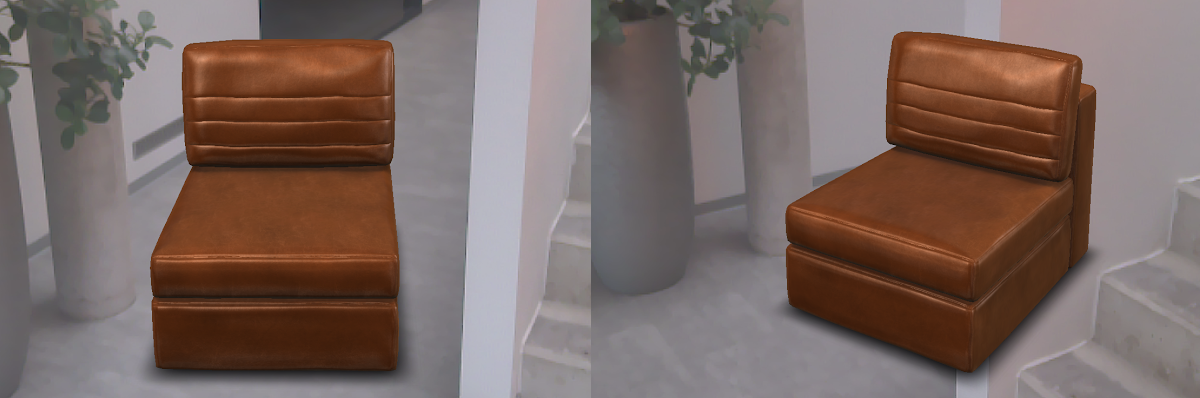
\includegraphics[width=1.0\textwidth]{content/images/occlusion-problem.png} 

  \caption{AR Projektion mit Project Tango - Links: Erfolgreiche Projektion. Rechts: Fehlerhafte Darstellung ohne Überdeckung.}
  \label{fig:occlusion-problem}
\end{figure}

Die Verfügbarkeit der Tiefeninformationen bei Project Tango könnte die Interaktionen oder Darstellungen in einer Augmented Reality Anwendung präziser an die echten räumlichen Gegebenheiten anpassen. Es existieren zum Beispiel prototypische Anwendungen, in denen virtuelle Markierungen passend an echten Objekten im virtuellen Raum positioniert werden können, indem sie auf die aktuellen Tiefeninformation des Sichtbereichs zurückgreifen. Eine weitere Idee ist es, Überlagerungen virtueller Objekte ermitteln zu können, an denen sich reale Objekte im Vordergrund befinden.

\section{Zielsetzung und Vorgehen}

Diese Arbeit will die Fragestellung beantworten, durch welche Verfahren mithilfe der Tiefeninformationen von Project Tango, automatisch und in Echtzeit die Überdeckung virtueller Objekte mit realen Objekten in einer Augmented Reality Szene realisiert werden kann. Dabei soll Project Tango als autonomes System betrachtet werden, welches diese Problemstellung selbstständig und mit den eingeschränkten Ressourcen dieser mobilen Plattform lösen soll.

Hierzu sollen zunächst bestehende Verfahren zur Bestimmung einer Augmented Reality Überdeckung durch eine Literaturrecherche gefunden werden. Diese Verfahren sollen dabei auf Ihre Anwendbarkeit mit der Project Tango Hardware überprüft werden. Sollten sich aus der Recherche weitere Ideen ergeben, wie speziell auf der Project Tango Hardware eine Überdeckung umgesetzt oder verbessert werden kann, sollen diese mit in die Arbeit eingebunden werden. Eine Idee könnte zum Beispiel sein, auch das Farbbild der normalen Kamera von Project Tango in die Optimierung der virtuellen Überlagerung einfließen zu lassen. Die identifizierten Verfahren sollen hiernach entsprechend implementiert werden, um sie darauf folgend in einer Testumgebung gegenüber zu stellen.

Strukturell wird in dieser Arbeit in Kapitel \ref{sec:thema} erst einmal auf die thematischen Grundlagen zu Augmented Reality und Project Tango eingegangen. Hier werden auch die existierenden Verfahren zur AR Überdeckung angesprochen. Unter Kapitel \ref{sec:algorithms} sind theoretische Grundlagen zu finden, die bei der späteren Umsetzung verschiedener Verfahren angewendet werden. Kapitel \ref{sec:optimization} beinhaltet die Argumentation und Beschreibung der gewählten Verfahren, welche unter Kapitel \ref{sec:implementation} auf der Project Tango Hardware umgesetzt werden. In Kapitel \ref{sec:evaluation} werden die vorliegenden Umsetzung in einem Testszenario gegenübergestellt, um eine Aussage treffen zu können, welcher Ansatz auf der Hardware oder für einen bestimmten Einsatz gut funktionieren könnte.



\chapter{Theoretische Vorbemerkung}

Im ersten Teil dieses Kapitels werden zunächst einmal die Grundlagen zu Augmented Reality beschrieben, wie diese Technologie einzuordnen ist, welche technischen Anforderungen ein Augmented Reality System hat und wo typische Einsatzszenarien liegen.


\section{Augmented Reality}

Augmented Reality (AR) ist eine Klasse aus dem Realitäts-Virtualitäts-Kontinuum von \cite{milgram1995augmented}, zu finden in Abbildung \ref{fig:virtual-continuum}, welche reale und virtuelle Objekte in einer realen Umgebung kombiniert. Diese virtuellen Objekte sind in der realen Umgebung idealerweise fest lokalisiert und fügen sich somit in das reale Erscheinungsbild ein. Typischerweise sind AR Anwendungen interaktiv, und stellen die virtuellen Objekte in Echtzeit und dreidimensional in der realen Welt dar. Für die Definition von AR Anwendungen gibt es zudem keine Limitierung für die Darstellungstechnologie, wie zum Beispiel das Projekt Tango Tablett oder einem Head-Mounted Display. AR beschränkt sich zudem nicht auf den angesprochenen Sinn - so sind zum Beispiel AR Anwendungen mit visueller, taktiler oder sogar olfaktorischer Umsetzung möglich.\\

Virtuel Reality (VR) oder auch Virtual Environment hingegen kapselt sich von der realen Umgebung ab und bietet Interaktionen in reinen virtuellen Umgebungen. VR konnte sich im Gegensatz zu AR deutlich schneller Entwickeln, da die technologischen Anforderungen an AR deutlich höher sind. \citep{van2010survey}\\

\begin{figure}
  \centering
	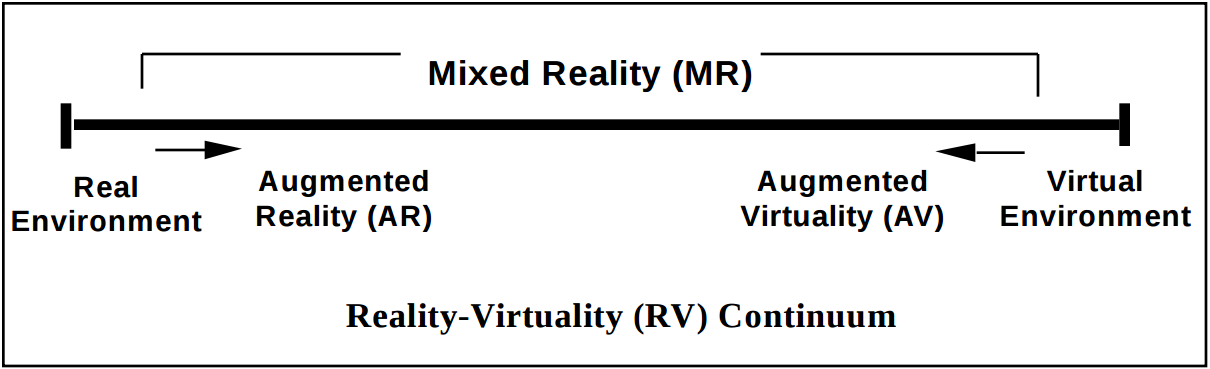
\includegraphics[width=0.85\textwidth]{content/images/theory/virtual-continuum.png} 
  \caption{Vereinfachte Darstellung des Realitäts-Virtualitäts-Kontinuum von \citet*{milgram1995augmented}}
  \label{fig:virtual-continuum}
\end{figure}

\subsection{Technische Anforderungen}

Dieser Abschnitt widmet sich den technischen Anforderungen an Augmented Reality, indem die potentiellen Display Technologien beschrieben werden, mögliche Trackingverfahren erläutern werden und zuletzt die Systeme bestimmt werden, mit denen ein Nutzer mit dem AR System interagieren kann.\\

\subsubsection{Display Technologie}

Der erste wichtige Teil der technologischen Anforderungen an AR sind visuelle Anzeigen (visual displays), welche sich nach \citet{van2010survey}
in diesem Anwendungsfall zunächst in drei Arten der Darstellung unterteilen und zudem unterschiedlich positioniert werden können. Die einfachste und günstigste Art der visuellen Darstellung in AR ist \enquote{video see-through}, wodurch die reale Umgebung durch eine Video Aufnahme ersetzt wird und die virtuellen Objekte digital in die Video Aufnahme gerendert werden. Das bietet außerdem die Möglichkeit Objekte aus der realen Umgebung zu entfernen oder zu ändern oder anhand der Luminanz Information vom Video das Rendering der virtuellen Objekte entsprechend an die Realität anzupassen.\\

Die nächste Möglichkeit zur Darstellung ist \enquote{optical see-through}, wodurch die virtuellen Objekte durch transparente Spiegel in das Sichtfeld des Betrachters gebracht werden. Anders als bei \enquote{video see-throught} bleibt die reale Auflösung für die visuelle Aufnahme des Betrachtes gleich und es können zudem keine Latenzprobleme beim Ändern des Betrachtungswinkels auftreten (parallax-effect).\\

Die dritte Möglichkeit ist die projizierte Darstellung, in der die Augmented Reality Überlagerung auf die realen Objekte projiziert werden. Diese Darstellung ermöglicht die Abdeckung vom gesamten Sichtfeld, benötigt aber eine entsprechende Kalibrierung bei Umgebungsänderungen.\\

Neben der Art der Darstellung können die Display Technologien laut \citet{azuma2001recent} anhand Ihrer Positionierung klassifiziert werden. Man unterscheidet zwischen am Kopf befestigten Displays (head-mounted), tragbare Displays (hand-held) und räumlich positionierten Displays. Zu jeder dieser Displayarten gibt es wiederum unterschiedliche technische Umsetzungen mit ihren spezifischen Vor- und Nachteilen bezüglich ihrer Anwendungsszenarien.\\

\subsubsection{Tracking Technologien}

Um eine virtuelle Projektion im realen Raum zu realisieren muss zunächst die Position und gegebenenfalls relative Positionsänderung des Displays bestimmt werden, auch \enquote{augmented reality registration} genannt. Man spricht dabei üblichweise von den \enquote{six degrees of freedom (6DOF)}, der Position im Raum (x, y, z) und der Orientierung (yaw, pitch, roll). \\

Frühe Techniken für die Registrierung benötigten üblicher Weise eine speziell vorbereitete Räumlichkeit, denn sie basierten auf mechanischen, magnetischen oder Ultraschall Sensoren um die Position zu bestimmen. Diese Sensoren sind zwar immer noch im Einsatz und bilden auch den Grundstein für AR und VR Forschung, sind aber praktisch gesehen zu komplex und aufwändig für die meisten Anwendungsfälle. \citep{van2010survey} \\

Für ein grobes Positions-Tracking, vor allem auch außerhalb von Gebäuden wird GPS genutzt. Für großräumliche Anwendung ist GPS, mit einer Varianz von 10-15 Metern und in Kombination mit einem Kompass, durchaus praktikabel. Zum Beispiel um sichtbare Flugzeuge oder Sterne visuell aufzubereiten. Innerhalb von Gebäuden basiert die grobe Positionierung laut \citet{van2010survey} oft auf verfügbaren Wifi Access Points oder RFID Markern. \citet{lamarca2005place} demonstrieren hierzu auch die Möglichkeit diese Technologie für grobe Lokalisation außerhalb von Gebäuden einzusetzen.\\

Optische Tracking Verfahren basierend auf Bildverarbeitung bieten laut \citet{van2010survey} deutlich genauere Resultate als die zuvor beschriebenen Verfahren. Es gibt hier viele verschiedene sensorische Ansätze ein optisches Tracking zu realisieren. Frühe verfahren nutzten referenzielle Marker oder Licht emittierende LEDs in einem vordefinierten Modell, um zwischen aufgenommenen Bildern eine homographische Transformation zu berechnen und um somit Rückschlüsse auf die Rotation und Positionsänderung der Kamera zu ziehen. Neue Verfahren ohne Marker nutzen Techniken zur Feature Detection und Matching um Referenzen und Bewegungen zwischen aufgenommenen Bildern zu bestimmen.\\

Viele kommerzielle und erfolgreiche Tracking Verfahren beruhen jedoch auf hybride Ansätze indem Sensoren kombiniert werden um potentielle Fehleinschätzungen eines Sensors oder einer Technik auszuschließen. So werden zum Beispiel Neigungssensor, Kompass und Gyroskop mit einem optischen Verfahren kombiniert um ein Tracking der sechs Freiheitsgrade zu optimieren. \citep{van2010survey}\\

\citet{azuma2001recent} erwähnt an dieser Stelle auch die Kalibrierung der Sensoren, die für ein präzises Registrieren nötig ist. So müssen zum Beispiel die Linseneigenschaften der Kamera für optisches Tracking bekannt sein, damit die Verfahren mit Krümmungen oder Verzerrungen umgehen können. Diese Informationen sind auch bei video see-through Displays für ein korrektes Projezieren der 3D Objekte wichtig. Zudem wird erwähnt, dass man Messfehlern oder Drifts der Position zum Beispiel mit der Zunahme von Gyroscop Informationen entgegenwirken kann, indem man auf Ereignisse wie einen Schritt des Nutzers wartet. \citep{azuma2001recent} \\

\subsubsection{Interaktions Technologien}

*

\subsection{Anwendungsbereiche}

* 

\chapter{Implementierung} \label{sec:implementation}

Dieses Kapitel widmet sich der Umsetzung der in Kapitel \ref{sec:optimization} beschriebenen Verfahren. Hierfür wurden im Laufe dieser Arbeit verschiedene Prototypen entwickelt, die jeweils als Proof of Concept für die einzelnen Verfahren galten. Ziel dieser Umsetzung ist es einen einzigen Prototypen in Form einer App auf dem Project Tango Gerät zu entwickeln, die den gesamten Funktionsumfang, welcher in Kapitel \ref{sec:final_prototype} zusammengefasst wird, beinhaltet. \\

Zudem muss ein Programmfluss geschaffen werden, der es ermöglicht, in die Daten des Tiefenbuffers mit eigenen Implementierungen eingreifen zu können, um ein Filtern zu ermöglichen. Wie das technisch ermöglicht wird, und auf welcher Basis die Anwendung implementiert wird, beschreibt das Kapitel \ref{eq:technic}. Hiernach werden die Umsetzung der die jeweiligen Verfahren näher erläutert.

\section{Finaler Prototyp} \label{sec:final_prototype}

Der finale Prototyp soll, wie bereits erwähnt, alle zuvor beschriebenen Verfahren zur Realisierung von Überlagerungen in einer Augmented Reality Szene beinhalten. Also muss zunächst eine einfache AR Szene geschaffen werden, in der eine virtuelle Kamera existiert, die die intrinsischen und extrinsischen Eigenschaften der realen Project Tango Kamera zu jeder Zeit entspricht. Außerdem muss das aktuelle Farbbild der RGB Kamera in der Szene im Hintergrund dargestellt werden. Für diese Aufgaben existieren, wie bereits in Kapitel \ref{sec:theory_project_tango} erwähnt, Schnittstellen, die diese Informationen liefern. 

Um eine reale Überdeckung sinnvoll testen zu können, benötigen wir zudem ein virtuelles Objekt in der Szene. Dieses sollte im Idealfall nicht zu einfach gestaltet sein, damit die Verfahren anhand praxisnaher Gegebenheiten verglichen werden können. Zu diesem Zweck sollen Objekte in die App geladen werden können, die in dem Forschungsbereich der Computergraphik typischerweise eingesetzt werden. Typische Modelle sind zum Beispiel der \enquote{Utah Teapot}, \enquote{Stanford Bunny} oder \enquote{Blenders Suzanne}\footnote{List of common 3D test models - \url{https://goo.gl/MsOtSW} (26.02.16)}.  Eines dieser Modelle soll in die Szene geladen werden und es soll die Möglichkeit gegeben sein, dass das Objekt flexibel positioniert werden kann. Um das zu realisieren, wird der beschriebene Raypicking Mechanismus für die Auswahlgeste umgesetzt.

Um die Ergebnisse der realen Überlagerung einfach gegenüberstellen zu können, sollen die beschriebenen Tiefenbild generierenden Verfahren flexibel im Betrieb ausgetauscht werden. Dazu gehört das Rendering der Pointcloud Projektion, die TSDF Rekonstruktion durch Chisel und die Ebenenrekonstruktion. Außerdem soll das Filtern des Tiefenbildes mit Hilfe des Guided Filter optional zu jeder Zeit möglich sein. Hilfreich wäre es zudem, die Einstellungen des Guided Filters flexibel anpassen zu können. Wie diese Verfahren und der flexible Austausch umgesetzt wird, wird in den folgenden Kapiteln näher beschrieben.

\section{Technische Umsetzung und Struktur} \label{eq:technic}

Wie bereits erwähnt, basiert das Project Tango System auf Googles Android Betriebsystem. Dies ermöglicht es Anwendungen mit bestehenden und bewährten Technologien wie OpenGL, Rajawali\footnote{Android OpenGL ES 2.0/3.0 Java Engine - \url{https://goo.gl/r9Ohdj} (27.02.16)} oder der Unity Engine entwickeln zu können. Project Tango bietet hierfür drei verschiedene Schnittstellen, in C/C++, Java und Unity (Mono Framework in C\#), um auf die Sensordaten in verschiedenen Umgebungen zugreifen zu können. Im Laufe dieser Arbeit wurden alle Schnittstellen mit verschiedensten prototypischen Entwicklungen getestet.

Der finale Prototyp wurde letztendlich in C/C++ entwickelt und basiert auf dem Android NDK\footnote{Android Native Development Kit - \url{http://goo.gl/ananZT} (27.02.16)}. Außerdem greifen die anderen, höher angesiedelten Schnittstellen auf genau die selbe native Implementierung zurück, um sie in Java und Unity zur Verfügung zu stellen. Außerdem ermöglicht die native Entwicklung, neben Performancevorteilen, den vollen Zugriff auf OpenGL Mechanismen, die von Rajawali (der OpenGL Java Abstraktion) gegebenenfalls ausgeschlossen werden. 

Das Project Tango Team stellt für die native Entwicklung die eigentliche Tango Schnittstellen Bibliothek\footnote{Project Tango C API - \url{https://goo.gl/lbBfAp} (27.02.16)}, eine Support-Bibliothek\footnote{Project Tango C Suppport API - \url{https://goo.gl/VGyeKm} (27.02.16)} und eine einfache Kapselung für OpenGL Anwendungen mit dem Namen TangoGL\footnote{TangoGL Repository - \url{https://goo.gl/ymDCsJ} (27.02.16)} an. Die Support-Bibliothek bietet verschiedene Hilfsfunktionen zur Datenverarbeitung und Allokation. TangoGL wiederum erleichtert den Einstieg in die OpenGL Entwicklung und übernimmt die grundlegende Struktur und Interoperabilität zu Project Tango. Zum Beispiel gibt es Methoden, um Tango Positionsdaten in eine Translationsmatrix umrechnen zu können oder Klassen, die das Rendern der aktuellen RGB Kamera Textur übernehmen. 

Abbildung \ref{fig:structure} zeigt grob den strukturellen Aufbau der Android Applikation. Der obere Teil der Grafik bezieht sich dabei auf den in Java implementierten Teil, der die Nutzeroberfläche, ihre Interaktion und den Renderingcanvas beinhaltet. Die Activity stellt jedoch nur einen kleinen Teil der Anwendung dar, denn alle Interaktionen und Ereignisse werden über ein Java Native Interface (JNI) zum nativen Teil der Anwendung geleitet, welcher die Ansprache der Schnittstellen, die Prozesslogik und das Rendering selbst beinhaltet. 

\begin{figure}[h]
  \centering
	\includegraphics[width=1.0\textwidth]{content/images/implementation/uml.png} 
  \caption{Struktureller Aufbau des Prototypen}
  \label{fig:structure}
\end{figure}

Die Hauptklasse \enquote{ARApp} in der Grafik widmet sich in der Anwendung nur der Anreicherung und Weiterleitung von JNI Informationen und der Ansprache der Project Tango Schnittstelle. Kern der Anwendung ist die \enquote{Scene} Klasse, welche die Sensorinformationen an das entsprechend aktive Verfahren zur Tiefenbild\-generierung weiterreicht. So wird zum Beispiel die Pointcloud an das Chisel, Pointcloud oder Plane Drawable weitergereicht, damit sie ein aktualisiertes Tiefenbild rendern oder die Rekonstruktion anreichern können. Auch das Farbbild der Kamera gelangt über die Scene zum RGB Drawable, welches letztendlich als eine texturierte Fläche am Ende des Kamera Frustum dargestellt wird. Die Szene selbst ermöglicht durch den Einsatz von OpenCV\footnote{Open Source Computer Vision - \url{http://opencv.org/} (26.03.16)} den optionalen Filter Prozess durch den Guided Filter. Um das zu ermöglichen wird ein OpenGL Framebuffer eingesetzt. Die Abbildung \ref{fig:rendering-process} zeigt hierzu das Vorgehen beim Rendering der Szene mit Hilfe des zusätzlich eingesetzten Framebuffer (TB). Um den Z-Buffer Ausschluss, also die letztendliche Überlagerung zu nutzen, muss der OpenGL Depth-Test aktiviert werden.


\begin{figure}[h]
  \centering
	\includegraphics[width=1.0\textwidth]{content/images/implementation/process.png} 
  \caption{Prozessdiagramm für das Rendering der Szene}
  \label{fig:rendering-process}
\end{figure}

\section{Umsetzung der Verfahren} \label{sec:method-implementation}

\subsubsection*{Tiefe aus der Pointcloud Projektion}

Wie im Kapitel \ref{sec:pc-projection} erwähnt müssen die Punkte der Project Tango Pointcloud auf die Bildebene projiziert werden und mit einer entsprechenden Tiefenfarbe und einem Radius auf den Tiefenpuffer gezeichnet werden. Dieser Schritt wurde auch bereits in Prototoypen mit den angegebenen Gleichungen umgesetzt. 

Nach dem das Proof of Concept jedoch fertig gestellt wurde ist aufgefallen, dass OpenGL neben dem Rendering von Polygonen auch primitiven wie Punkte und Linien unterstützt. Somit konnten die Punkte im finalen Prototyp einfach vor die Kamera positioniert werden und mit Hilfe der symbolischen Konstante \enquote{GL\_POINTS} anstelle von \enquote{GL\_TRIANGLES} gerendert werden. Zudem lässt sich durch einen entsprechenden Vertexshader die Größe der Punkte anpassen. Abbildung \ref{fig:pc-demo} zeigt links die optionale gefärbte Projektion auf der Bildebene und rechts das resultierende Tiefenbild.

\begin{figure}[h]
  \centering
	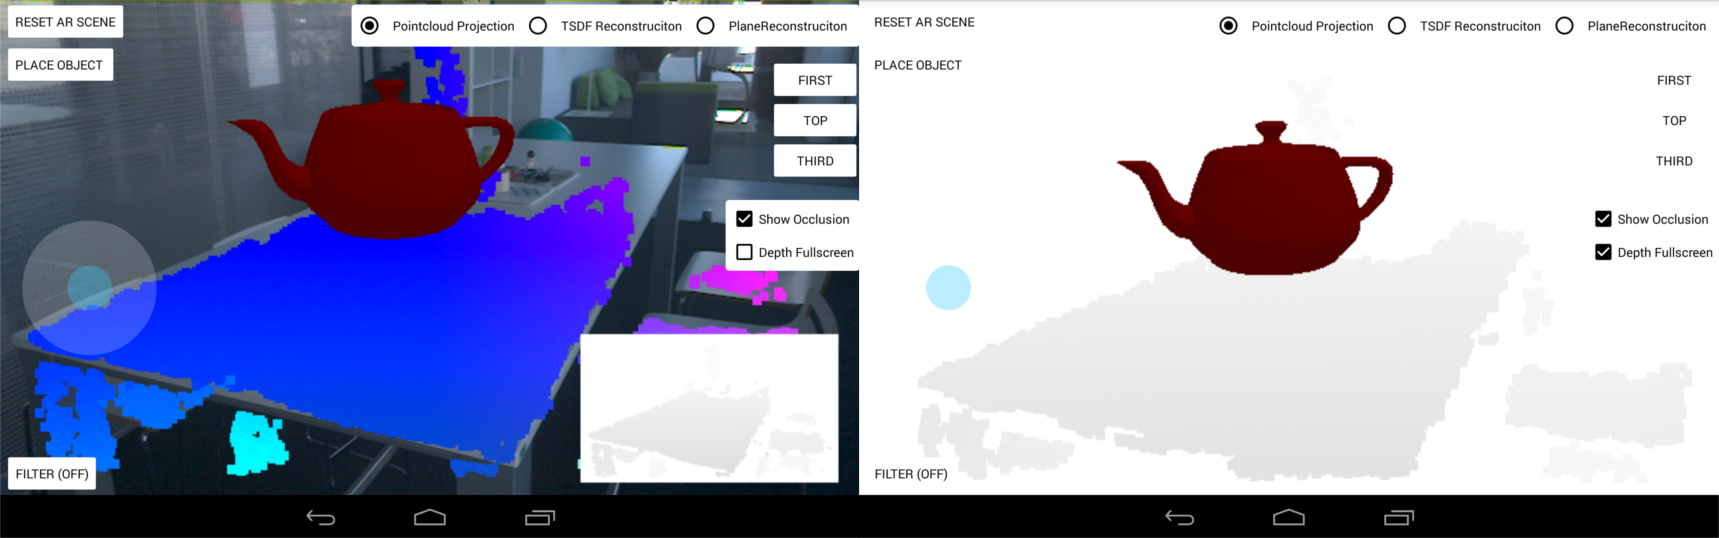
\includegraphics[width=1.0\textwidth]{content/images/implementation/pc-demo.png} 
  \caption{Pointcloud Projektion Prototyp. Links optionale Projektion auf der Bildebene. Rechts das resultierende Tiefenbild.}
  \label{fig:pc-demo}
\end{figure}



\subsubsection*{Planare Rekonstruktion}

Der erste Proof of Concept der planaren Rekonstruktion wurde zu Beginn dieser Arbeit auf Java Ebene implementiert und entwickelte sich nach und nach zu dem in \ref{sec:plane-reconstruction} beschriebenen Verfahren. Für die finale Umsetzung in dem nativen Prototypen mussten somit alle Algorithmen und Datenstrukturen neu in C/C++ umgesetzt werden. Begonnen wurde mit dem Octree, der in seinen tiefsten Zweigen die Menge aller aufgenommenen Punkte für den jeweiligen Sektor und eine Instanz der \enquote{Reconstructor} Klasse beinhaltet. Diese beinhaltet alle beschriebenen Algorithmen zur Ebenen Rekonstruktion wie RANSAC, die linearen Regression und den Graham Scan. 

\begin{figure}[h]
  \centering
	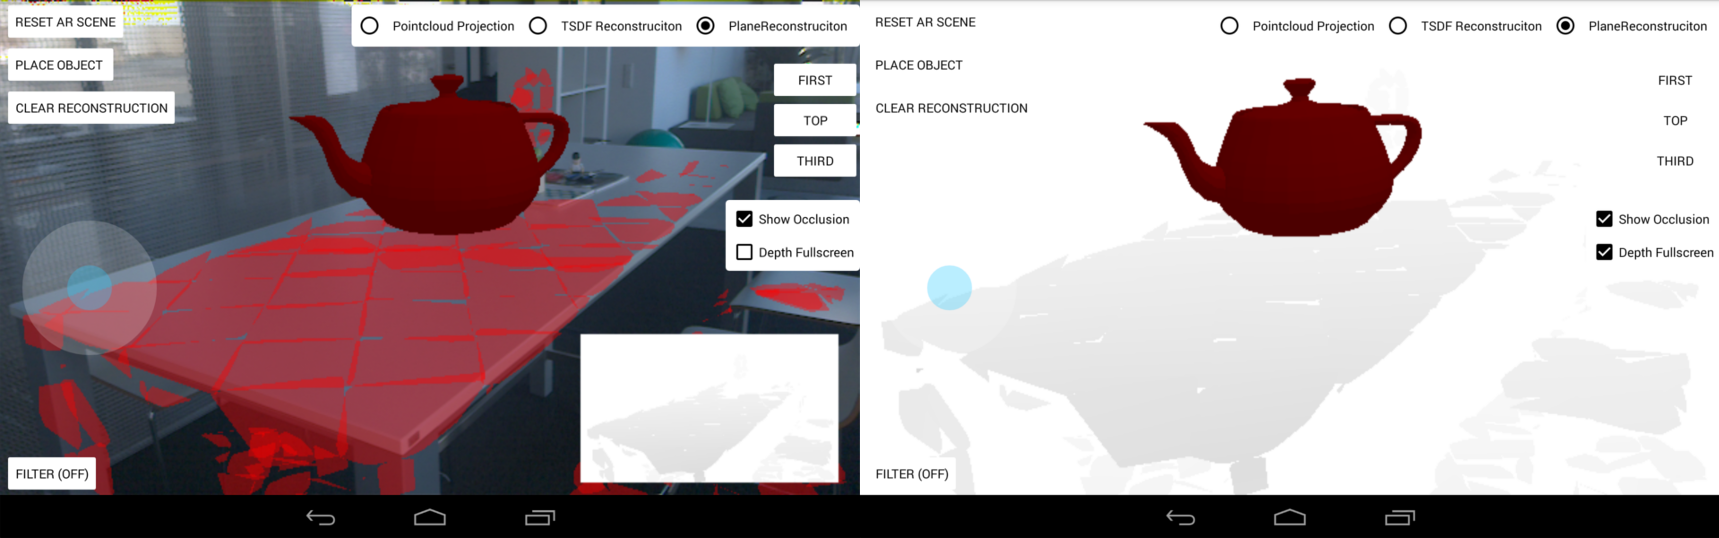
\includegraphics[width=1.0\textwidth]{content/images/implementation/plane-demo.png} 
  \caption{Planare Rekonstruktion Prototyp. Links optionale Projektion auf der Bildebene. Rechts das resultierende Tiefenbild.}
  \label{fig:plane-demo}
\end{figure}

Für die Berechnung mit Vektoren und Matrizen wurde wie auch im gesamten Projekt die OpenGL Mathematics Bibliothek (GLM)\footnote{OpenGL Mathematics - http://goo.gl/2oY83s (27.02.16)} verwendet. Sie bietet typische Primitiven mit entsprechenden Operationen für Berechnungen der linearen Algebra. Wie bereits beschrieben wird für die lineare Regression die Berechnung von Eigenvektoren mit ihren Eigenwerten benötigt. Diese Berechnung wird von GLM nicht unterstützt. Hier wurde die Eigen-Bibliothek\footnote{Eigen: template library for linear algebra - http://goo.gl/TsNOuW (27.02.16)} verwendet, die diese Operation für den Anwender anbietet. Abbildung \ref{fig:plane-demo} zeigt die Ergebnisse der Ebene Rekonstruktion links und der daraus Resultierenden Tiefeninformation rechts.


\subsubsection*{TSDF Rekonstruktion}

\citet{Klingensmith_2015_7924} erwähnen, dass ihr Verfahren Chisel zunächst als proprietäre Umsetzung im Project Tango Constructor\footnote{Project Tango Constructor - https://goo.gl/8HdTnY (27.02.16)}, Googles Demo Anwendung zur räumlichen Rekonstruktion, umgesetzt wurde. Zu Ihrer Publikation haben sie jedoch zusätzlich eine Open-Source ROS basiertes Modul zur Verfügung gestellt. Diese Bibliothek mit dem Namen OpenChisel\footnote{OpenChisel - Chisel chunked TSDF library - https://goo.gl/nla8hy (27.02.16)} wurde für den Prototypen in dieser Arbeit auf das Android NDK portiert. Dafür wurden einige Module des C++11 Standards, wie zum Beispiel \enquote{st::shared\_ptr}, die zum derzeitigen Kenntnisstand vom Android NDK nicht unterstützt oder dessen Umsetzung ein anderes Verhalten aufweist, auf die Boost\footnote{Boost C++ Libraray - http://www.boost.org/ (27.02.16)} Implementationen abgeändert. Neben der Boost Bibliothek nutzt OpenChisel auch die Eigen Bibliothek für Primitiven und Berechnungen der linearen Algebra.

Als Eingabe benötigt OpenChisel neben der Kameraposition und Kameraeigenschaften entweder einer Pointcloud oder ein Tiefenbild. In der Proof of Concept Umsetzung war erkennbar, dass OpenChisel mit der Pointcloud von Project Tango deutlich schlechtere Ergebnisse lieferte, als die Implementation des Constructors von Google. Dadurch, dass die Support Bibliothek von Google seit Februar 2016 eine performante Methode\footnote{TangoSupport\_upsampleImageNearestNeighbor - https://goo.gl/mchIie (27.02.16)} anbietet, um aus einer Punktewolke eine DepthMap mit einer Auflösung von \(320x180\) Pixel zu interpolieren, wird nun ein Tiefenbild für OpenChisel verwendet. Die resultierenden Ergebnisse kommen dadurch der Constructor Implementation deutlich näher. Abbildung \ref{fig:chisel-demo} zeigt eine exemplarische Rekonstruktion einer Pointcloud links mit dem resultierenden Tiefenbild rechts.

\begin{figure}[h]
  \centering
	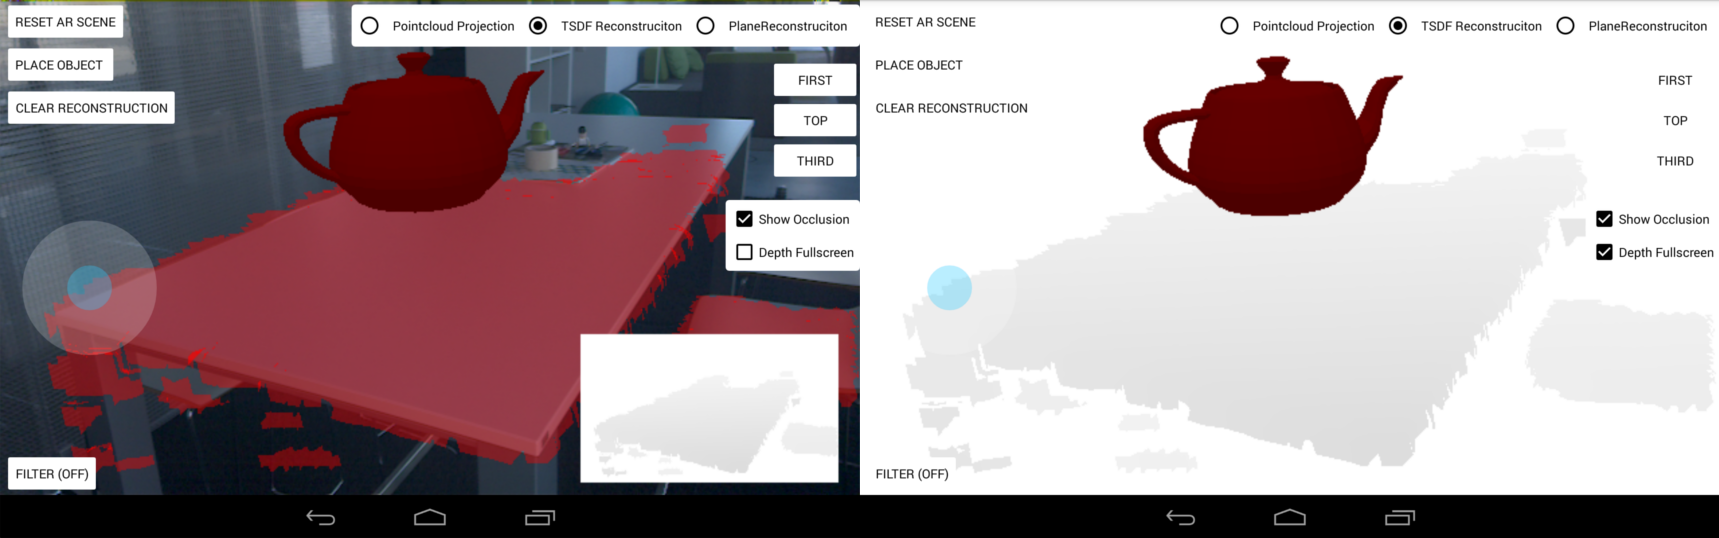
\includegraphics[width=1.0\textwidth]{content/images/implementation/chisel-demo.png} 
  \caption{OpenChisel Rekonstruktion Prototyp. Links optionale Projektion auf der Bildebene. Rechts das resultierende Tiefenbild.}
  \label{fig:chisel-demo}
\end{figure}


\subsubsection*{Guided Filter}

Für die Anwendung des Guided Filters wurde, wie bereits erwähnt, die Computer Vision Bibliothek OpenCV verwendet. Um diesen Filter mit OpenCV anwenden zu können mussten zuvor das RGB Bild und das Tiefenbild in das OpenCV Format gebracht werden. Dies war jedoch mit den Methoden \enquote{glReadPixels} und \enquote{glTexImage2D} für den aktuell selektierten Framebuffer und der OpenGL Textur problemlos möglich. Zwar sind die Speicherkonventionen von OpenGL und OpenCV, was die X und Y Achse angeht, genau vertauscht, jedoch ist das Filtern, welches daraus folgend gedreht stattfindet, für den Nutzer völlig intransparent und kann dadurch ignoriert werden.

Problematisch ist jedoch, dass das OpenGL Tiefenbild eine Farbtiefe von 16Bit nutzt und der OpenCV Guided Filter nur auf 8Bit Graustufen angewendet werden kann. Diese Transformation und die daraus resultierende Ungenauigkeit der Tiefe wurde jedoch zunächst in Kauf genommen, da erst einmal der Mechanismus als solches getestet werden soll. In der späteren Auswertung von Testszenarien muss diese Transformation berücksichtigt werden. 

Diese Implementierung ermöglicht es, den Guided Filter dynamisch auf das aktuell generierte Tiefenbild mit dem aktuell aufgenommen RGB Bild als Leitbild anzuwenden. Außerdem lassen sich die Filter Parameter, dem Radius \(r\) und den Einflussfaktor \(\epsilon\) dynamisch variieren. Abbildung \ref{fig:filter-demo} zeigt das Tiefenbild der TSDF Rekonstruktion links, auf die rechts der Guided Filter mit dem aktuellen RGB Bild angewendet wurde. 

\begin{figure}[h]
  \centering
	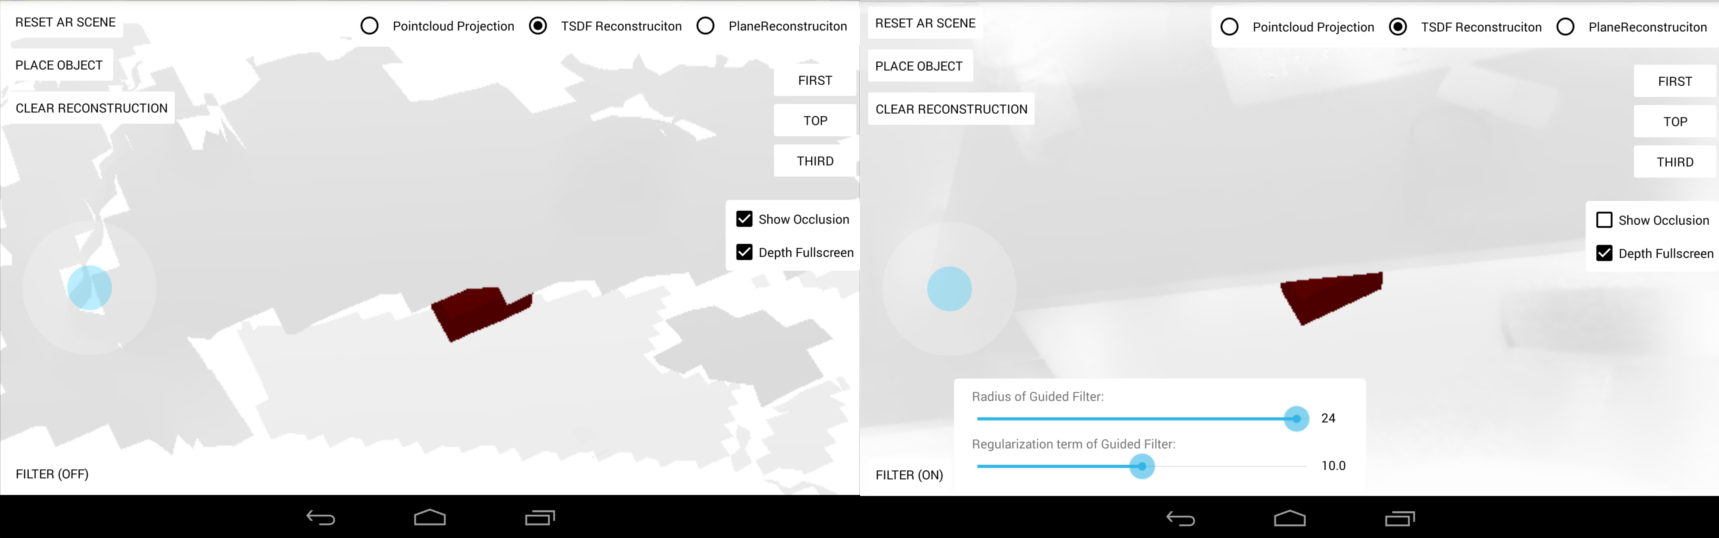
\includegraphics[width=1.0\textwidth]{content/images/implementation/filter-demo.png} 
  \caption{Anwendung des Guided Filters auf eine TSDF Rekonstruktion. Links vor und rechts nach der Anwendung.}
  \label{fig:filter-demo}
\end{figure}


\section{Technische Problemstellungen}

Auch wenn schon einige Probleme in der Umsetzung der jeweiligen Verfahren in Kapitel \ref{sec:method-implementation} näher beschrieben wurden, werden hier noch Einzelheiten aufgegriffen, die bei der Entwicklung für Projekt Tango zu beachten waren. 

Alle von Project Tango zurückgegebenen Vektoren besitzen ihre eigene Konvention bezüglich der Achsenanordnungen. Gegenüber der Konvention in OpenGL sind die Achsen \(Z\) und \(Y\) vertauscht. Außerdem zeigt die resultierende \(Z\)-Achse in die entgegengesetzte Richtung. Aufgrund dieser unterschiedlichen Konventionen müssen alle Vektoren \(\vec{v}\) von Project Tango mit der Transformationsmatrix \(T_{OGL}^{PT}\) aus Gleichung \ref{eq:transformation} konvertiert werden \citep{Proje15:online}. Nachdem Google im Laufe dieser Arbeit neue Schnittstellen\footnote{Project Tango API: Transformation Support - \url{https://goo.gl/N8dapq} (29.02.16)} zur Verfügung gestellt hat, um diese Transformationen zu abstrahieren, können die \enquote{TransformationSupport} Methoden hierfür genutzt werden.

\begin{equation} \label{eq:transformation}
T_{OGL}^{PT} =\left( \begin{matrix} 1&0&0&0\\0&0&-1&0\\0&1&0&0\\0&0&0&1 \end{matrix} \right)
\end{equation}

Wie bei vielen Echtzeitsystemen ist das Problem der Nebenläufigkeit (engl. Concurrency) auch in der Schnittstelle von Project Tango zu beachten. Die API von Project Tango publiziert die Sensordaten typischerweise asynchron. Außerdem werden die Rekonstruktionsverfahren von den entsprechenden API Publikationen angestoßen. Deshalb muss besonders beim Rendering sichergestellt werden, dass die Daten während dieses Prozesses nicht modifiziert werden. Diese Synchronisation wird durch den Einsatz von \enquote{std::mutex} aus der C/C++ Standard-Bibliothek gewährleistet. 

Bei der Anwendung des Guided Filters von OpenCV ist zu beachten, dass die  Speicherkonventionen von OpenGL und OpenCV, was die X und Y Achse angeht, genau vertauscht sind. Dadurch können zum Umwandeln der Bilder in das jeweilige Framework nicht die direkten Adressen verwendet werden, da sonst das Bild um \(90^{\circ}\) gedreht wird. Da dieser Filterprozess jedoch für den Nutzer völlig transparent durchgeführt wird und das Bild wieder in OpenCV zurück konvertiert wird, kann der Filterprozess einfach um \(90^{\circ}\) gedreht durchgeführt werden.





\appendix
\listoffigures            
\include{content/acknowlegements}
\chapter{Ergebnisaufnahmen}
\begin{sidewaysfigure}[h]
  \centering
	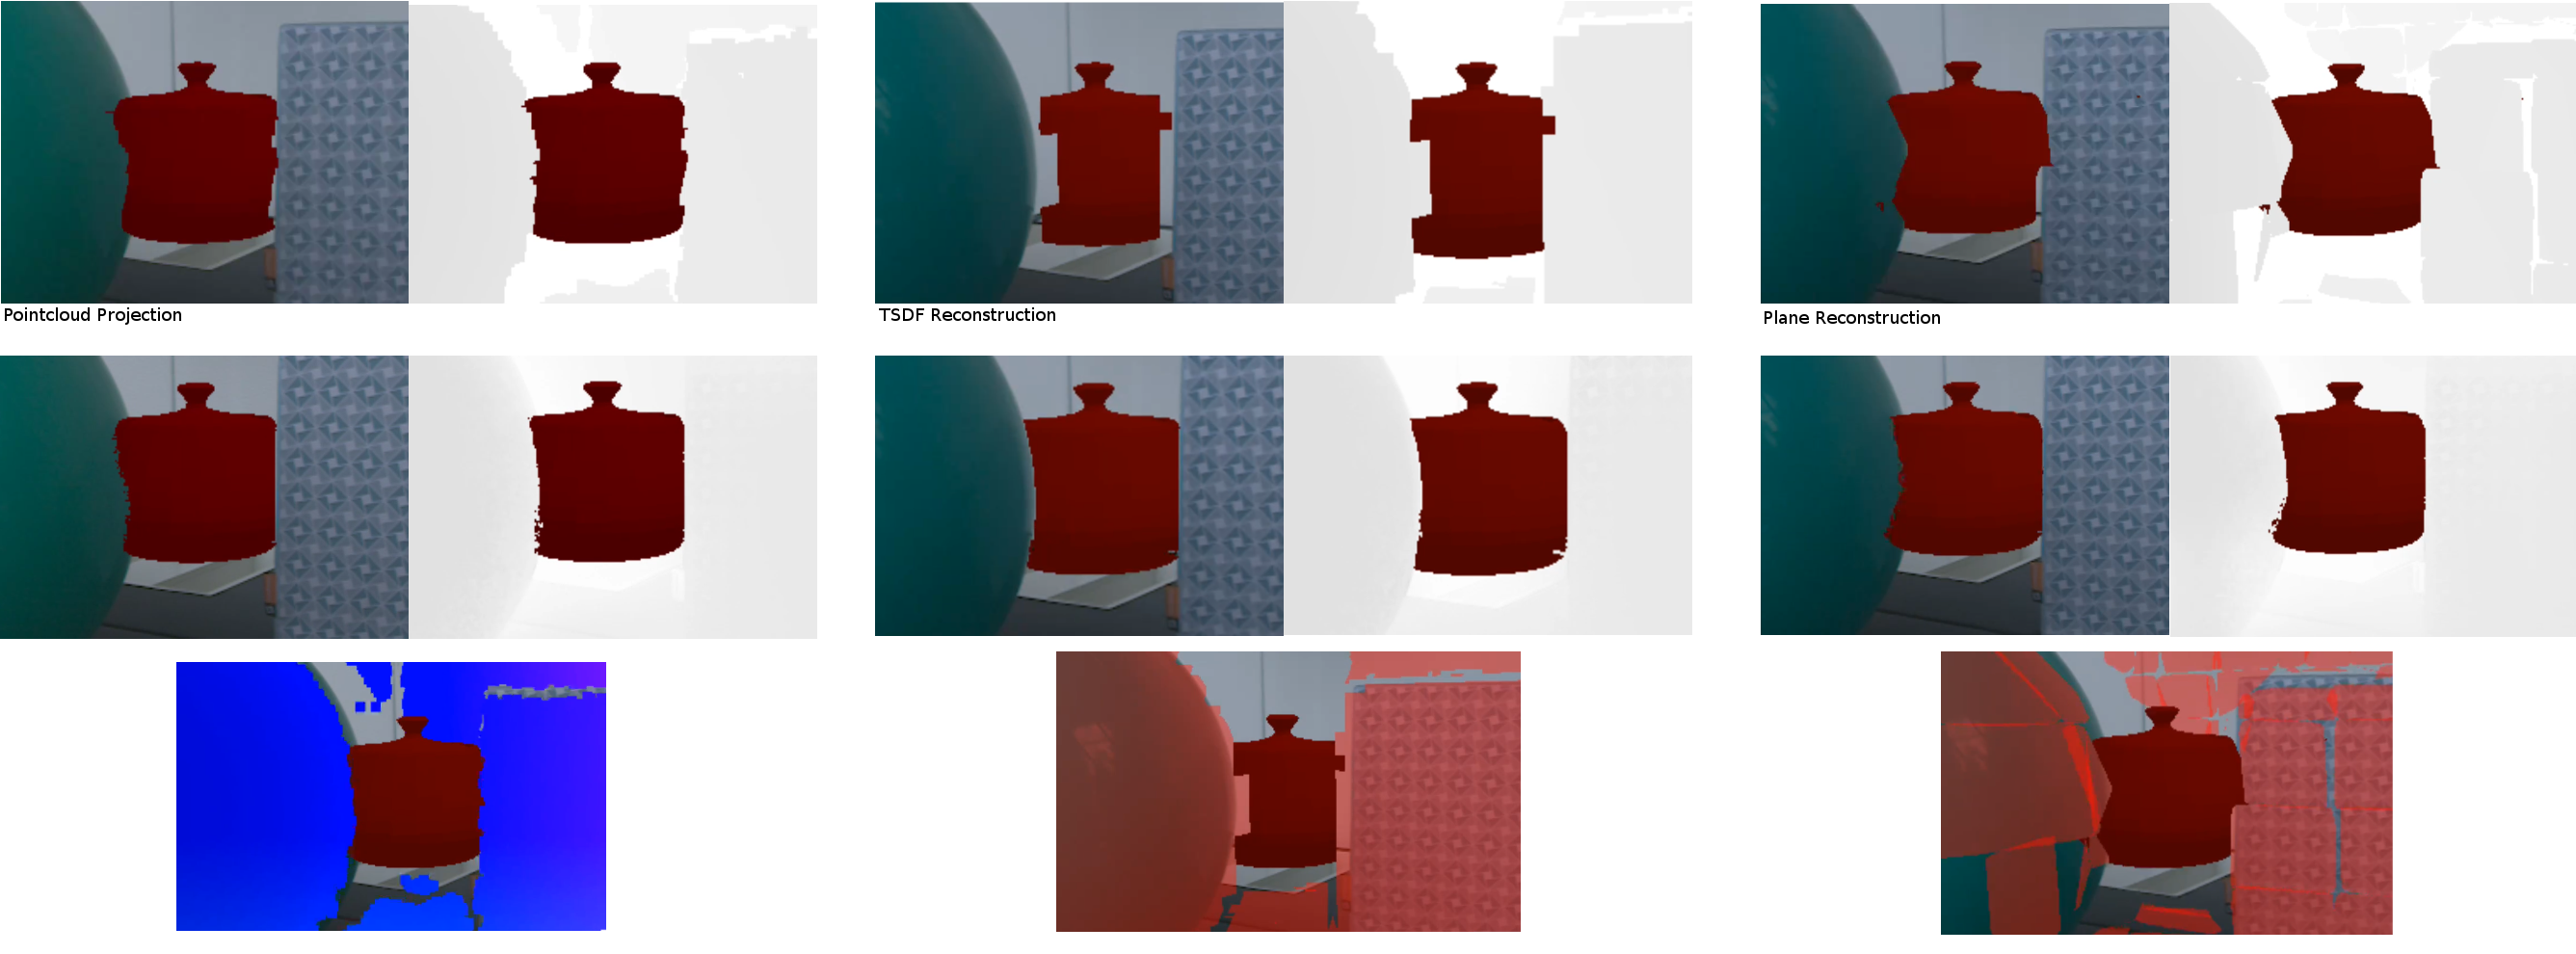
\includegraphics[width=1.0\textwidth]{content/images/evaluation/static_occlusion.png} 
  \caption{Ergebnisaufnahmen aus der ersten statischen Szene}
  \label{fig:static_occlusion}
\end{sidewaysfigure}

\begin{sidewaysfigure}[h]
  \centering
	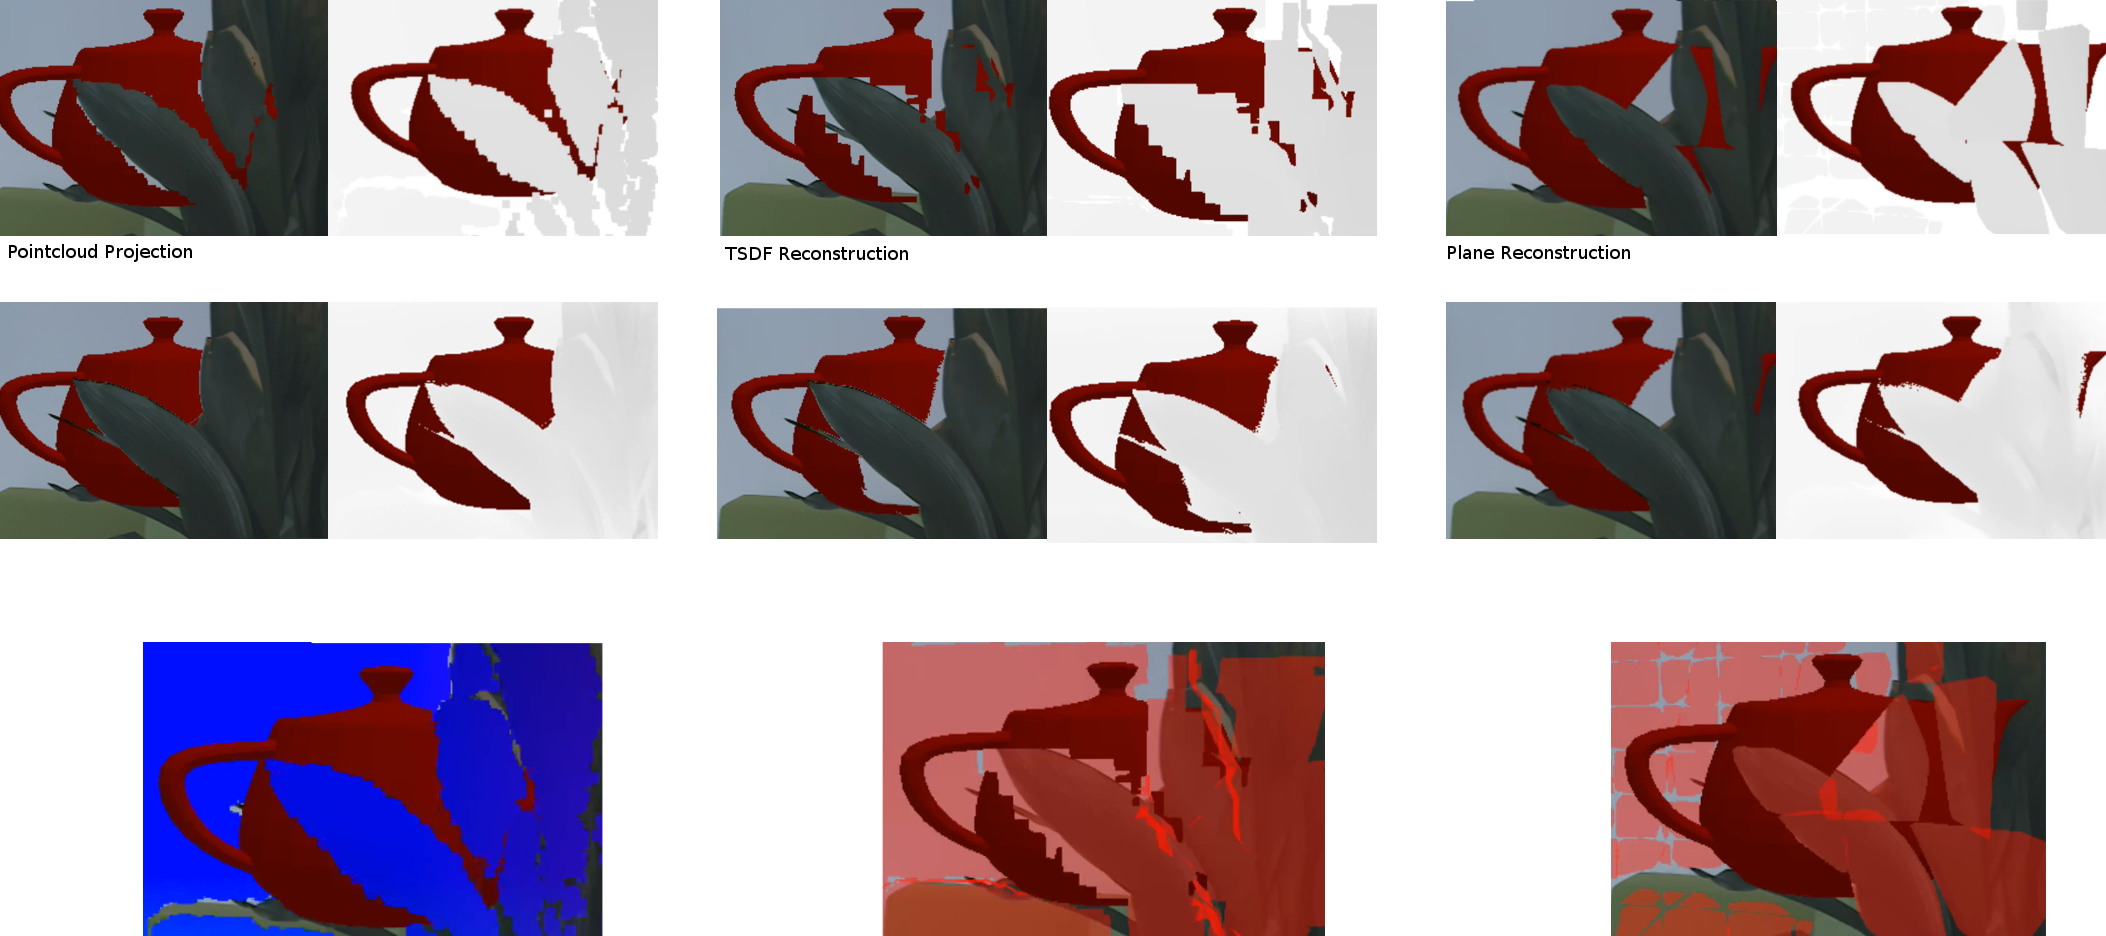
\includegraphics[width=1.0\textwidth]{content/images/evaluation/plant_occlusion.png} 
  \caption{Ergebnisaufnahmen aus der zweiten statischen Szene}
  \label{fig:plant_occlusion}
\end{sidewaysfigure}

\begin{sidewaysfigure}[h]
  \centering
	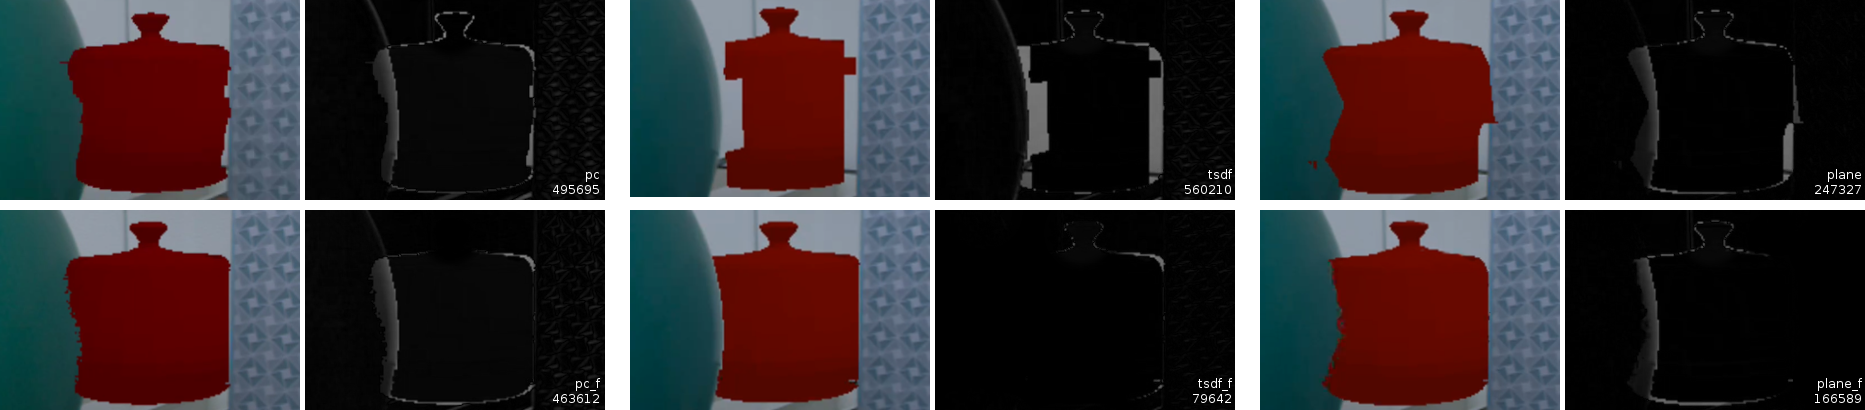
\includegraphics[width=1.0\textwidth]{content/images/evaluation/static_occlusion_results.png} 
	
\includegraphics[width=1.0\textwidth]{content/images/evaluation/spacer.png} 
	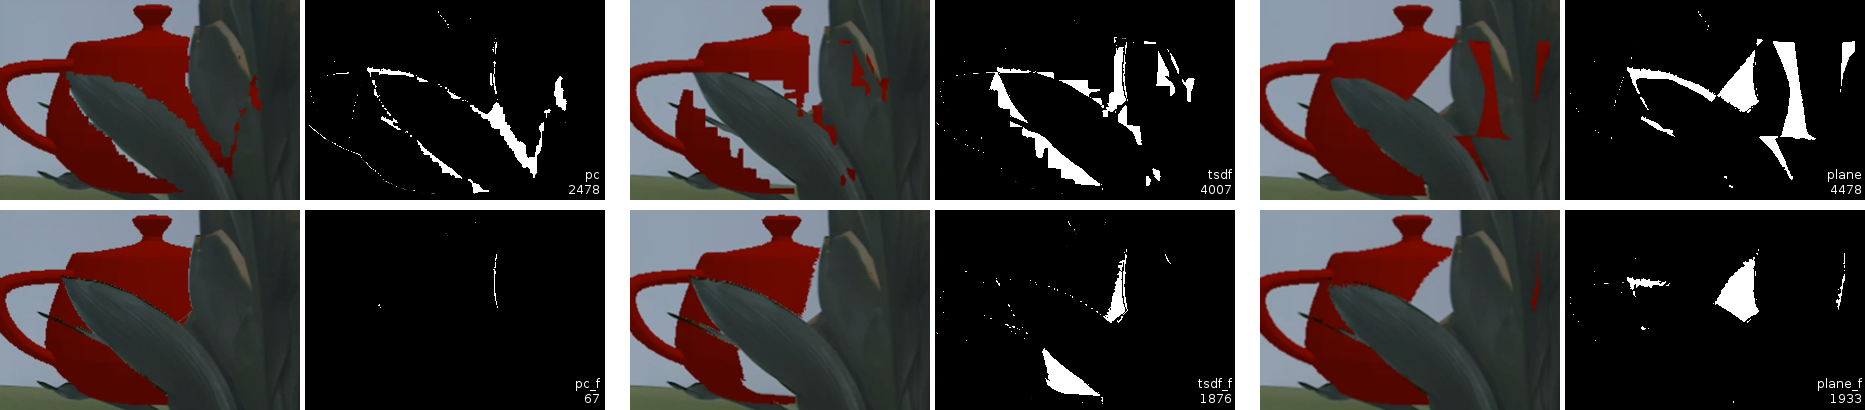
\includegraphics[width=1.0\textwidth]{content/images/evaluation/plant_occlusion_results.png} 
  \caption{Differenzbilder der Verfahren in ersten (oben) und zweiten Szene (unten)}
  \label{fig:static_occlusion_results}
\end{sidewaysfigure}



\addcontentsline{toc}{chapter}{Bibliography}

\bibliography{main}
\bibliographystyle{natdin} 

\end{document}

